%\pagebreak
\section{\kcode{stripe} Construct}
\label{sec:stripe}
\index{constructs!stripe@\kcode{stripe}}
\index{stripe construct@\kcode{stripe} construct}

Striping changes the order of logical iterations of a loop nest such that 
consecutive iterations become iterations executed with distances specified
by the \kcode{sizes(\plc{k1,k2..})} clause on the \kcode{stripe} construct.
The values in the distance list apply to the associated loops in the loop
nest, from outermost to innermost.
For a striping distance of \plc{k}, the execution starts with the first iteration,
then skips \plc{k-1} iterations, and continues with logical iteration \plc{k}, then 
skips next \plc{k-1} iterations, and so on until exceeding the logicial iteration space.
The execution continues with ``stripes'' starting with the second iterations,
until all logical iterations have been executed exactly once.

Some of the use cases of striping include:
\begin{itemize}
  \item Reordering to avoid false sharing of neighboring iterations
  in stencil computations,
  \item Matching GPU progress group sizes to improve performance.
\end{itemize}

\begin{figure}[H]
\begin{subfigure}[b]{.5\textwidth}
%\centering
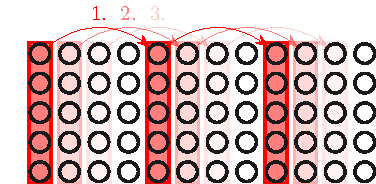
\includegraphics[width=0.8\textwidth]{figs/stripe-1d_striping}
\vspace*{2mm}
\caption{1-dimensional striping}\label{fig:1d_striping}
\end{subfigure}%
\begin{subfigure}[b]{.5\textwidth}
%\centering
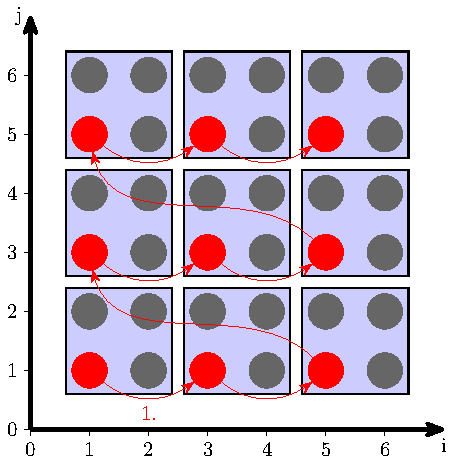
\includegraphics[width=0.8\textwidth]{figs/stripe-2d_tiling}
\caption{2-dimensional striping on a grid}\label{fig:2d_striping}
\end{subfigure}
\caption{Striping illustrations}\label{fig:striping}
\end{figure}

The following example shows 1-d striping of a single loop using
the \kcode{stripe} directive with the \kcode{sizes(\ucode{4})} clause
and its equivalent code
(see Figure~\ref{fig:striping}A for illustration).

\cexample[6.0]{stripe}{1}
\ffreeexample[6.0]{stripe}{1}

The following example shows 2-d striping of two nested loops using
the \kcode{stripe} directive with the \kcode{sizes(\ucode{2,2})} clause 
and its equivalent code
(see Figure~\ref{fig:striping}B for illustration).
The 2-dimensional striping effectively performs
tiling that partitions logical iterations into a ``grid.''
Striping executes one iteration of each tile in each stripe.
The logical iteration of the first tile represents the ``offset'' 
within each tile of the grid and can be seen as tiling followed by
a loop interleave, as illustrated by the equivalent code.

\cexample[6.0]{stripe}{2}
\ffreeexample[6.0]{stripe}{2}

